\chapter{\lr{Image Compression}}
اولین کاربرد مهم روش
\lr{SVD}
در کاهش سایز تصاویر
\footnote{
\lr{Image Compression}
}
می‌باشد.
در این بخش هدف دستیابی به تصویری با حجم کمتر و کیفیتی نزدیک به تصویر اصلی می‌باشد.
برای نمایش تصاویر، ابتدا از ماتریس‌
\lr{Gray scale}
استفاده کرده، و در آخر هم روی تصاویر رنگی این روش را تست می‌کنیم.


\section{شهود روش \lr{SVD} برای کاهش سایز}
تصویر سیاه و سفید زیر را در نظر بگیرید:

این تصویر را می‌توان با یک ماتریس
$A_{n \times m}$
نمایش داد که درایه های آن عددی بین 0(سیاه) و یک(سفید) اند.
فرض کنید تجزیه
\lr{SVD}
این ماتریس به فرم
$A=U \Sigma V^T$
باشد.
می‌دانیم
عناصر قطر
$\Sigma$
مقادیر ویژه‌ی این ماتریس
بصورت نزولی می‌باشد.
ایده‌ی اصلی
\lr{SVD}
برای کاهش سایز این ماتریس،
حذف مقادیر ویژه‌ی کم اهمیت است، به طوری که ماتریس حاصل تقریبی از همین ماتریس ولی با رنک کمتری باشد.



\section{پیاده سازی روش}
در این بخش به پیاده سازی این روش با پایتون می‌پردازیم. برای این پیاده سازی از کتابخانه های
\lr{numpy, matplotlib, Pillow}
استفاده شده.
کد مورد استفاده در این بخش در
\href{https://github.com/atrin-hojjat/svd-image-processing}{اینجا}
قابل دسترس است. برای اجرای کد یک
\lr{Virtual environment}
پایتون ساخته و
\lr{requirements.txt}
را نصب نمایید.
برای قطعه کد‌های استفاده شده
\lr{Jupyter Notebook}
آماده شده، برخی کد های نمودار ها در فایل پایتون مجزا قرار دارند.



\subsection{پیاده سازی روی تصاویر سیاه و سفید}
برای پیاده سازی این روش کاهش حجم، ابتدا از یک تصویر سیاه و سفید استفاده می‌کنیم. برای تبدیل تصویر به یک ماتریس از مقادیر سیاه و سفید از کد زیر استفاده می‌کنیم:

\begin{latin}
  \begin{python}
image_name = "cat"
image_path = "./cat.png"

from PIL import Image
import matplotlib.pyplot as plt
import numpy as np
import os

image = Image.open(image_path)

# Convert the image to grayscale (black and white)
bw_image = image.convert('L')
bw_image_array = np.array(bw_image)

plt.imshow(bw_image_array, cmap='gray')
plt.axis('off')
plt.show()

bw_image_array.shape
  \end{python}
\end{latin}

همانطور که مشاهده می‌کنید، این تصاویر را با یک ماتریس با مقادیر بین
$0$
تا
$256$
می‌توان نشان داد. در مرحله بعد، تجزیه
\lr{SVD}
این ماتریس را به دست ‌می‌اوریم


\begin{latin}
  \begin{python}
U, S, VT = np.linalg.svd(bw_image_array)
U.shape, S.shape, VT.shape
  \end{python}
\end{latin}

حال برای به دست آوردن یک تصویر کمتر، کافیست
$k$
مقدار بزرگ
$\Sigma$
را درنظر گرفته و بقیه را حذف کنیم:


\begin{latin}
  \begin{python}
compressed_image = U[:, :k] @ np.diag(S[:k]) @ Vt[:k]
  \end{python}
\end{latin}

حال می‌توانیم این تصویر را با تقریب‌های مختلف بررسی کنیم:


\begin{latin}
  \begin{python}
def compress_image(U, S, Vt, rank):
    return U[:, :rank] @ np.diag(S[:rank]) @ Vt[:rank]

def show_image(image):
    plt.imshow(image, cmap='gray')
    plt.axis('off')
    plt.show()

def save_grayscale_image(image_array, output_path):
    if image_array.dtype != np.uint8:
        image_array = image_array.astype(np.uint8)
    image = Image.fromarray(image_array, mode='L')
    image.save(output_path)
compression_ratios = [1, 4, 8, 16, 32, 64, 128, 256, 512, 750, 1000, 1024, 2048]
save_grayscale_image(bw_image_array, "cat-grayscale.png")
original_size = os.path.getsize("cat-grayscale.png")

rank_errors = []

for rank in compression_ratios:
    print("Rank", rank)
    image = compress_image(U, S, VT, rank)
    filename = f"cat-{rank}.png"
    save_grayscale_image(image, filename)
    result_size = os.path.getsize(filename)
    print(f"Size {result_size / 1024 / 1024:.2}Mb", )

    error = np.mean((image - bw_image_array) ** 2)
    print(f"Error {error}")
    rank_errors.append(error)
    show_image(image)


  \end{python}
\end{latin}

نتیجه‌ی کد با تقریب‌های مختلف را می‌توانید مشاهده‌کنید:

\begin{figure}
  
\includegraphics[width=\linewidth]{../image-compression/cat-1.png}
  \caption{$rank=1$}
  \label{fig:cat-bw-rank-1}
\end{figure}

\begin{figure}
  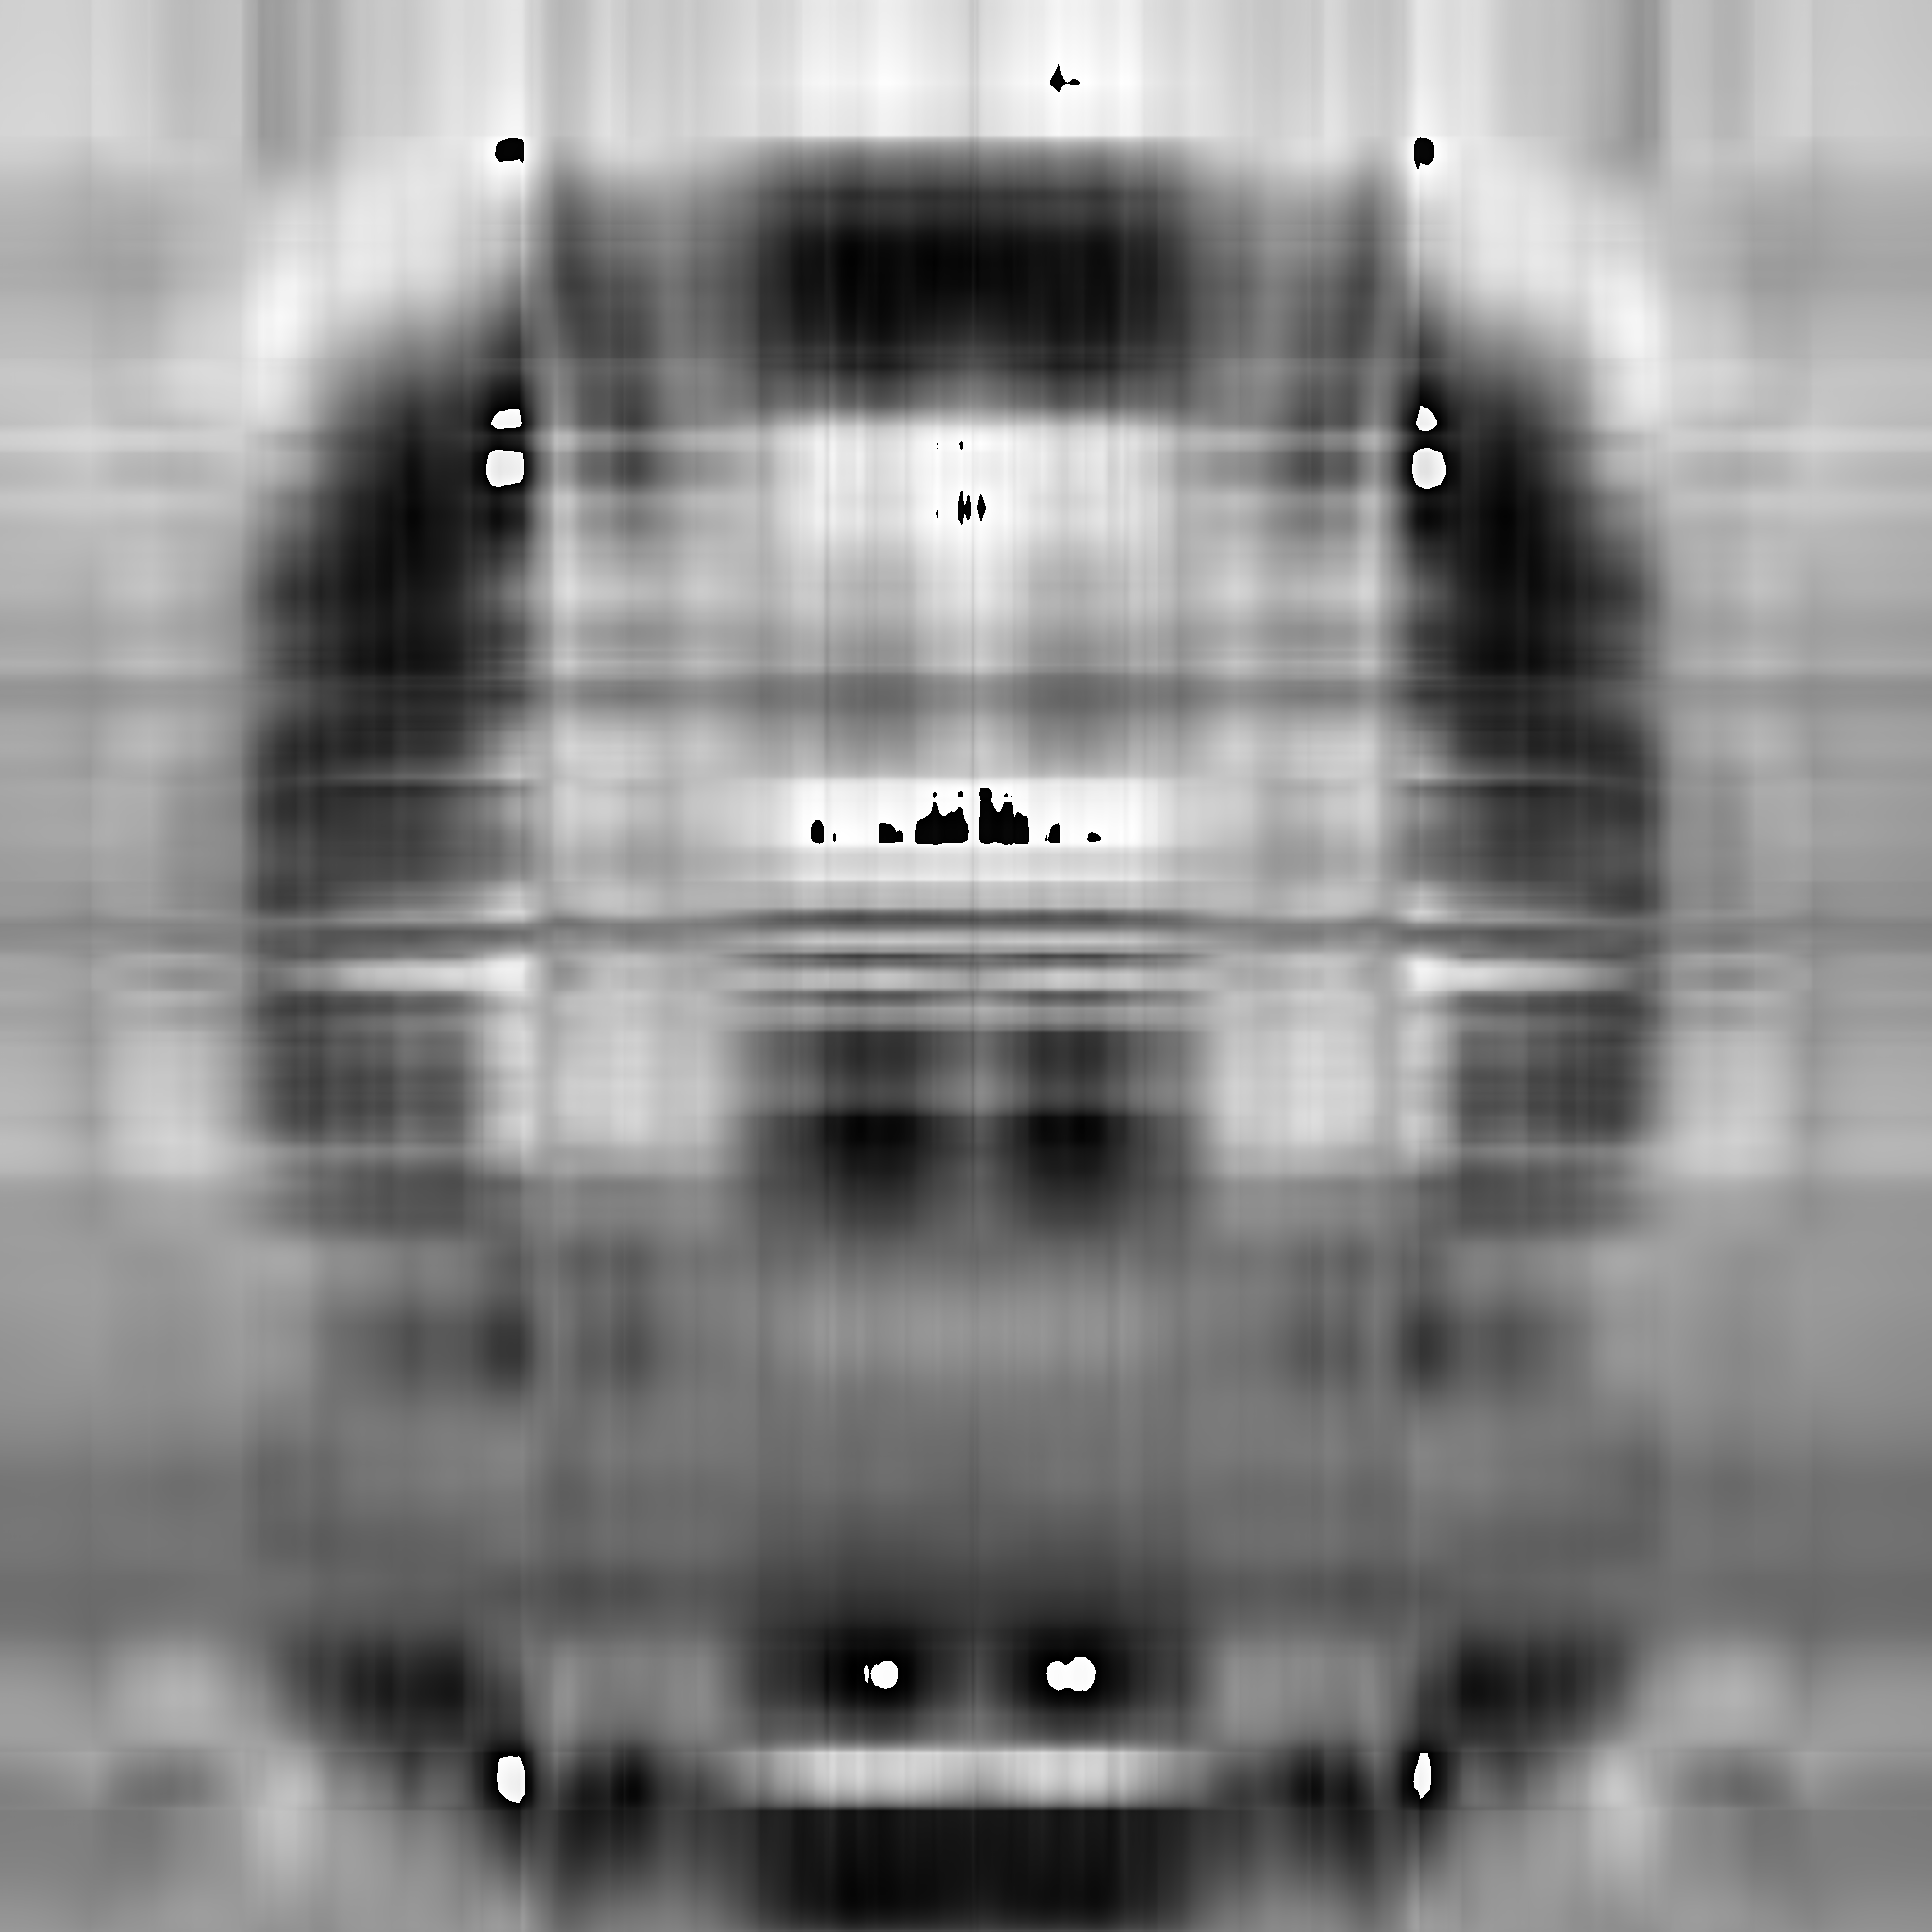
\includegraphics[width=\linewidth]{../image-compression/cat-4.png}
  \caption{$rank=4$}
  \label{fig:cat-bw-rank-4}
\end{figure}

\begin{figure}
  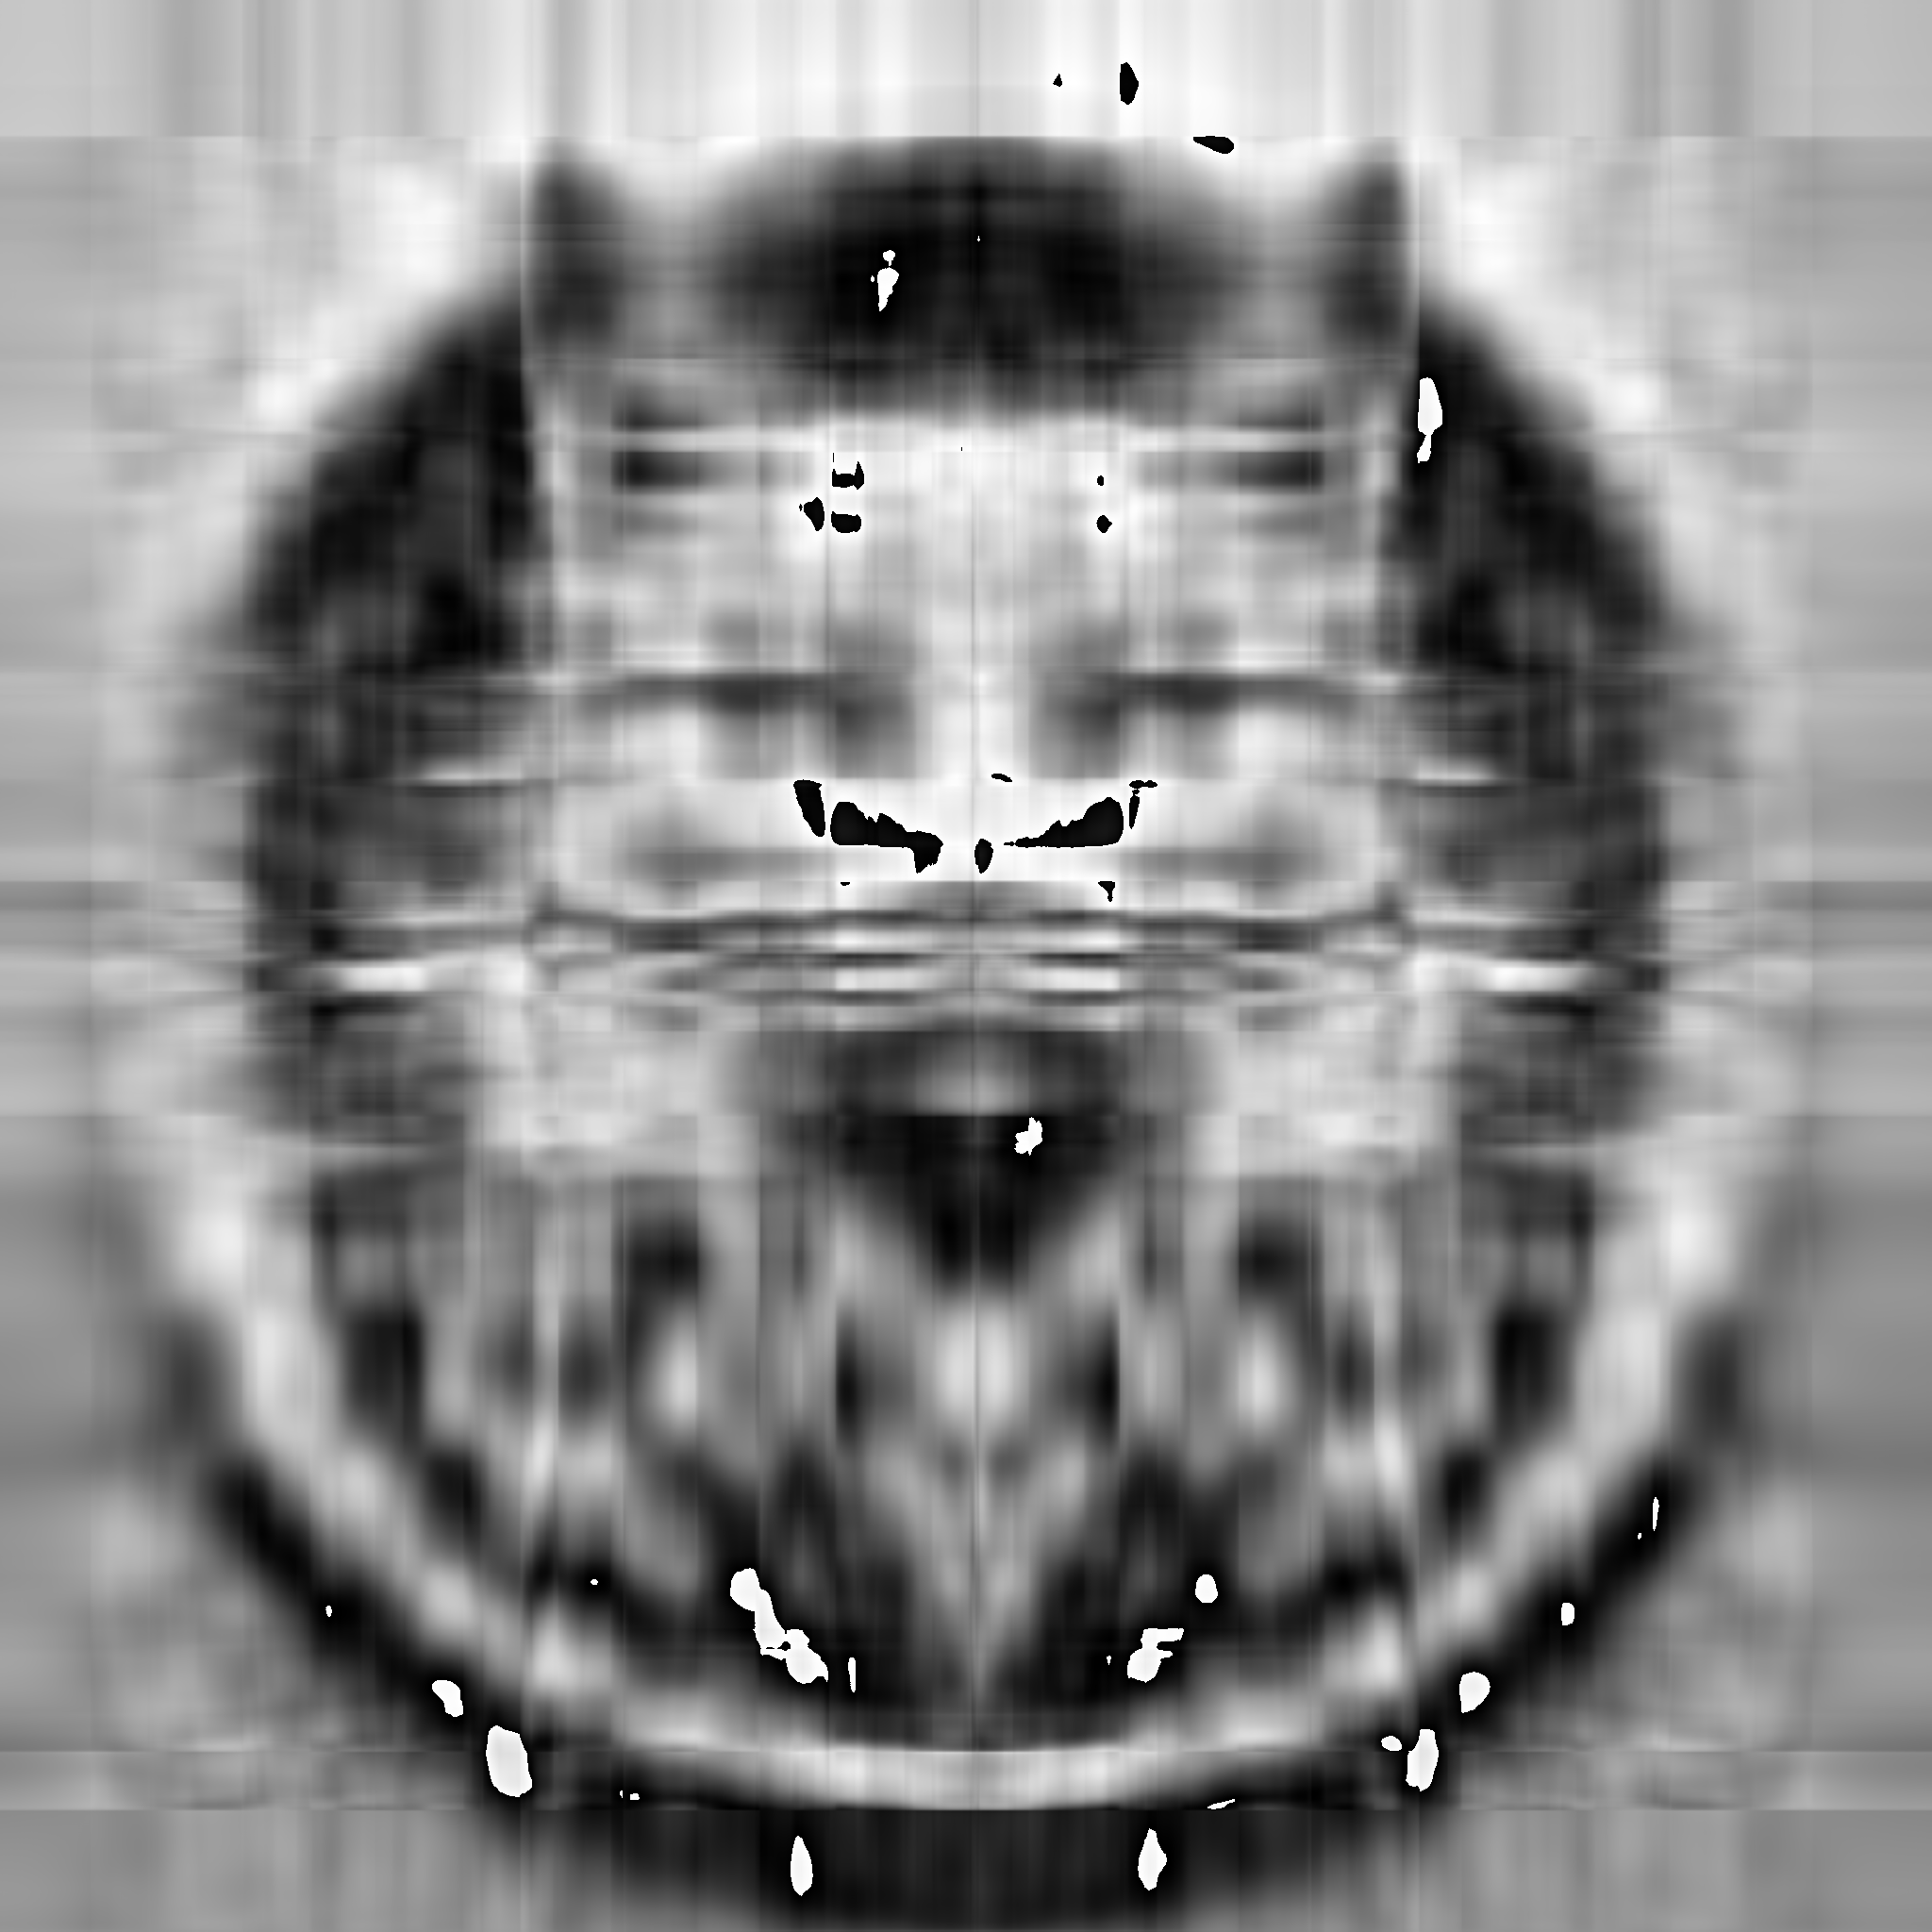
\includegraphics[width=\linewidth]{../image-compression/cat-8.png}
  \caption{$rank=8$}
  \label{fig:cat-bw-rank-8}
\end{figure}

\begin{figure}
  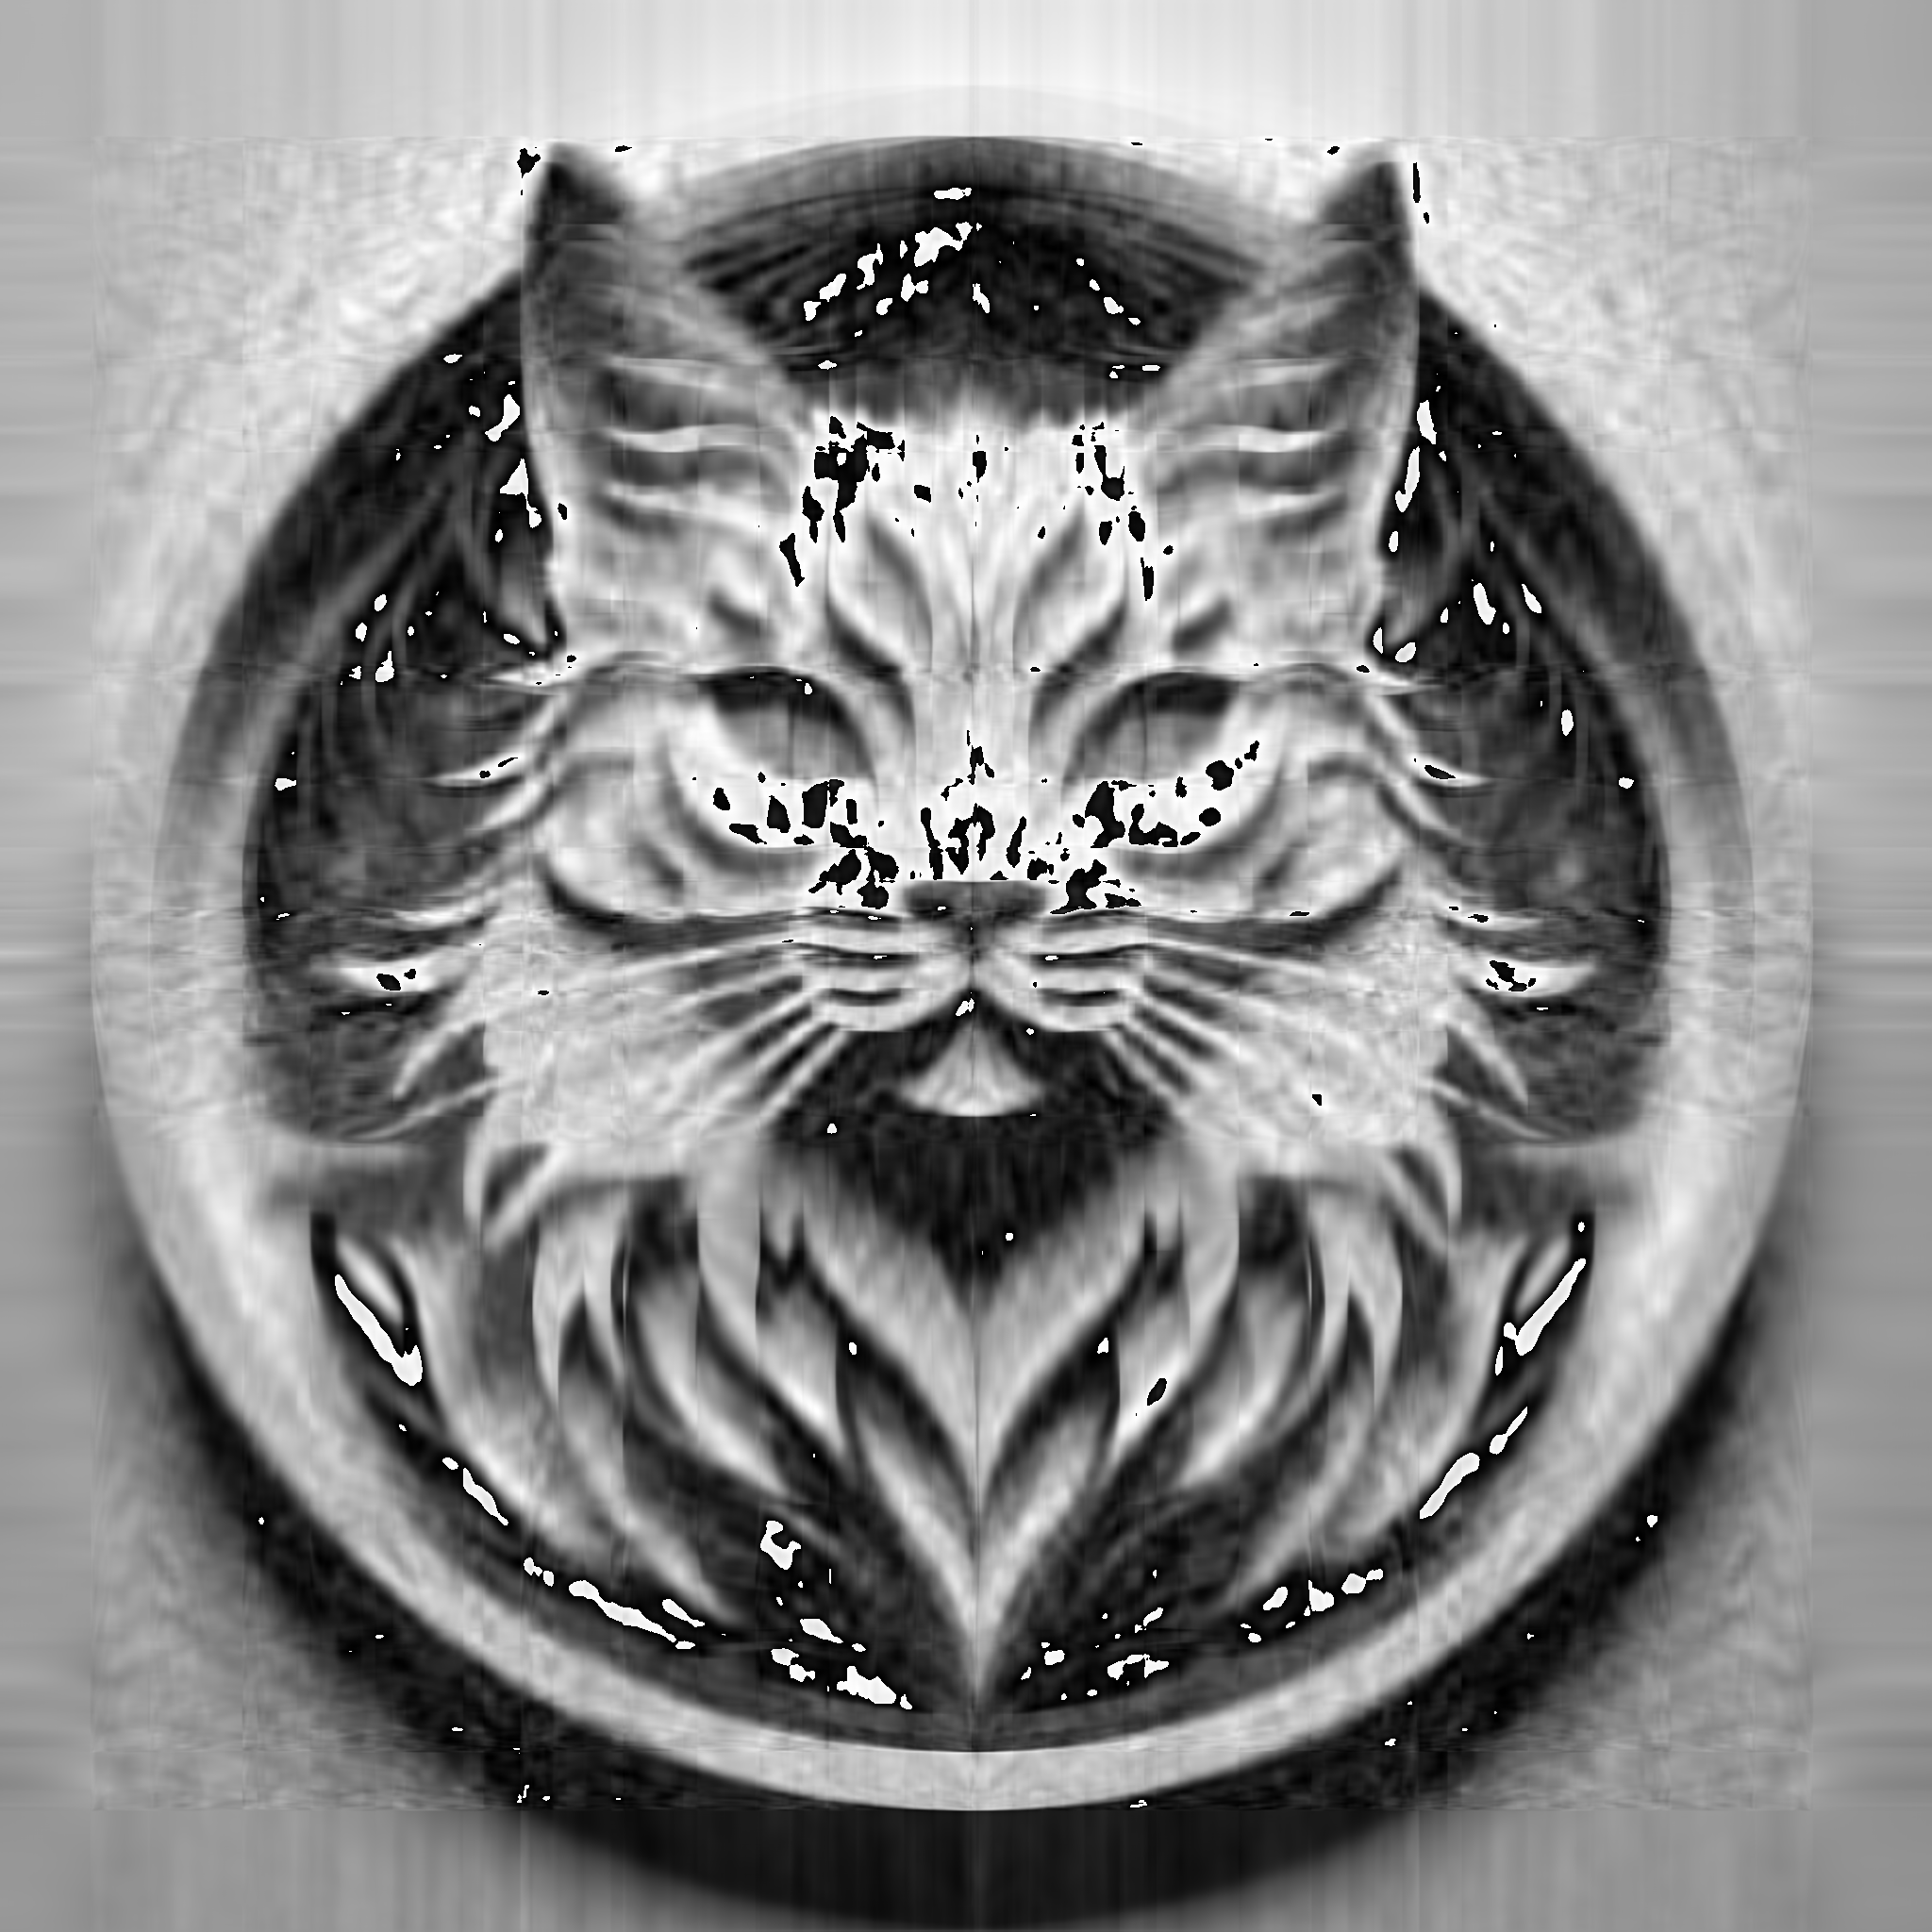
\includegraphics[width=\linewidth]{../image-compression/cat-32.png}
  \caption{$rank=32$}
  \label{fig:cat-bw-rank-32}
\end{figure}


\begin{figure}
  \includegraphics[width=\linewidth]{../image-compression/cat-256.png}
  \caption{$rank=256$}
  \label{fig:cat-bw-rank-256}
\end{figure}


\begin{figure}
  \includegraphics[width=\linewidth]{../image-compression/cat-1024.png}
  \caption{$rank=1024$}
  \label{fig:cat-bw-rank-1024}
\end{figure}

\begin{figure}
  \includegraphics[width=\linewidth]{../image-compression/cat-2048.png}
  \caption{$rank=2048$}
  \label{fig:cat-bw-rank-2048}
\end{figure}

همانطور که مشاهده می‌کنید، حتی در $rank$
پایین، کلیتی از تصویر دیده می‌شود، و با نزدیک شدن به سایز اصلی تصویر، تفاوت تقریبا ناچیز می‌باشد.

\subsection{بررسی خطا روش}
برای بررسی خطا در این روش
از دو معیار
\lr{MSE}
و
\lr{PSNR}
استفاده می‌کنیم.
\cite{4426357}
\cite{imcprichdavad}


برای محاسبه‌
$MSE$
یا
\lr{Mean Squared Error}
کافیست تفاوت تصویر نهایی به تصویر اولیه را محاسبه، و سپس مربعات ماتریس را میانگین بگیریم:

\begin{latin}
  \begin{python}
mse = np.mean((image - bw_image_array) ** 2)
  \end{python}
\end{latin}


معیار
$PSNR$
نشان دهنده‌ی میزان نویز به دیتا در تصویر می‌باشد.
روش حاسبه‌ی
$PSNR$
به شکل زیر می‌باشد:

\begin{equation}
  PSNR = 10 \log{10} \frac{255}{MSE}
\end{equation}


\begin{latin}
  \begin{python}
    psnr = 10 * (np.log10(255 / np.sqrt(mse)))
  \end{python}
\end{latin}


حال می‌توانیم این مقادیر را برای تقریب‌های مختلف محاسبه کرده و رسم کنیم:

\begin{latin}
  \begin{python}
from PIL import Image
import matplotlib.pyplot as plt
import matplotlib
import numpy as np
import os

image_name = "cat"
image_path = "./cat.png"

image = Image.open(image_path)

# Convert the image to grayscale (black and white)
bw_image = image.convert('L')
bw_image_array = np.array(bw_image)

U, S, VT = np.linalg.svd(bw_image_array)


def compress_image(U, S, Vt, rank):
    return U[:, :rank] @ np.diag(S[:rank]) @ Vt[:rank]


compression_ratios = [1, 4, 8, 16, 32, 64, 128, 256, 512, 750, 1000, 1024, 2048]

mse_values = []
psnr_values = []

for rank in compression_ratios:
    print("Rank", rank)
    image = compress_image(U, S, VT, rank)

    mse = np.mean((image - bw_image_array) ** 2)
    psnr = 10 * (np.log10(255 / np.sqrt(mse)))
    mse_values.append(mse)
    psnr_values.append(psnr)

plt.figure(figsize=(8, 6))
plt.plot(compression_ratios, mse_values, marker='o', color='blue', linestyle='-', linewidth=2, markersize=8)
plt.title('Mean Squared Error (MSE) vs. SVD compresssion')
plt.xlabel('Rank')
plt.ylabel('MSE')
plt.grid(True)
plt.tight_layout()
plt.savefig(os.path.join("../output", "image-comp-col-mse.jpg"))
matplotlib.rcParams.update({
    "pgf.texsystem": "xelatex",
    'text.usetex': True,
    'pgf.rcfonts': False,
    "font.family": "mononoki Nerd Font Mono",
    "font.serif": [],
    #  "font.cursive": ["mononoki Nerd Font", "mononoki Nerd Font Mono"],
})
plt.savefig(os.path.join("../output", "image-comp-col-mse.pgf"))
plt.show()

plt.figure(figsize=(8, 6))
plt.semilogx(compression_ratios, mse_values, marker='o', color='blue', linestyle='-', linewidth=2, markersize=8)
plt.title('Mean Squared Error (MSE) vs. log SVD compresssion')
plt.xlabel('Rank')
plt.ylabel('MSE')
plt.grid(True)
plt.tight_layout()
plt.savefig(os.path.join("../output", "image-comp-col-mse-log.jpg"))
matplotlib.rcParams.update({
    "pgf.texsystem": "xelatex",
    'text.usetex': True,
    'pgf.rcfonts': False,
    "font.family": "mononoki Nerd Font Mono",
    "font.serif": [],
    #  "font.cursive": ["mononoki Nerd Font", "mononoki Nerd Font Mono"],
})
plt.savefig(os.path.join("../output", "image-comp-col-mse-log.pgf"))
plt.show()

plt.figure(figsize=(8, 6))
plt.plot(compression_ratios, mse_values, marker='o', color='blue', linestyle='-', linewidth=2, markersize=8)
plt.title('PSNR vs. SVD compresssion')
plt.xlabel('Rank')
plt.ylabel('PSRN')
plt.grid(True)
plt.tight_layout()
plt.savefig(os.path.join("../output", "image-comp-psnr.jpg"))
matplotlib.rcParams.update({
    "pgf.texsystem": "xelatex",
    'text.usetex': True,
    'pgf.rcfonts': False,
    "font.family": "mononoki Nerd Font Mono",
    "font.serif": [],
    #  "font.cursive": ["mononoki Nerd Font", "mononoki Nerd Font Mono"],
})
plt.savefig(os.path.join("../output", "image-comp-col-psnr.pgf"))
plt.show()


plt.figure(figsize=(8, 6))
plt.semilogx(compression_ratios, mse_values, marker='o', color='blue', linestyle='-', linewidth=2, markersize=8)
plt.title('PSNR vs. log SVD compresssion')
plt.xlabel('Rank')
plt.ylabel('PSRN')
plt.grid(True)
plt.tight_layout()
plt.savefig(os.path.join("../output", "image-comp-col-psnr-log.jpg"))
matplotlib.rcParams.update({
    "pgf.texsystem": "xelatex",
    'text.usetex': True,
    'pgf.rcfonts': False,
    "font.family": "mononoki Nerd Font Mono",
    "font.serif": [],
    #  "font.cursive": ["mononoki Nerd Font", "mononoki Nerd Font Mono"],
})
plt.savefig(os.path.join("../output", "image-comp-col-psnr-log.pgf"))
plt.show()

  \end{python}
\end{latin}


\insertfig{../output/image-comp-mse.pgf}{\lr{MSE vs Rank}}{bw_comp_mse}
\insertfig{../output/image-comp-mse-log.pgf}{\lr{MSE vs log Rank}}{bw_comp_mse_log}
\insertfig{../output/image-comp-psnr.pgf}{\lr{PSNR vs Rank}}{bw_comp_psnr}
\insertfig{../output/image-comp-psnr-log.pgf}{\lr{PSNR vs log Rank}}{bw_comp_psnr_log}

همانطور که مشاهده میشود، بخش عمده بهینه سازی تا
$rank=256$
انجام میشود که حدود
$12.5\%$
ابعاد اصلی تصویر می‌باشد.


\subsection{پیاده سازی با تصاویر رنگی}
هر تصویر رنگی، شامل سه بخش
\lr{R, G, B}
می‌باشد که هریک نمایانگر میزان یکی از رنگ‌های قرمز، سبز،و آبی اند.
برای پیاده سازی این روش در یک تصویر رنگی، کافیست برای هر یک از
\lr{channel}
ها این پروسه‌را انجام دهیم، و سپس نتیجه هر سه را کنار یکدیگر قرار دهیم:



\begin{latin}
  \begin{python}
image_name = "cat"
image_path = "./cat.png"


from PIL import Image
import matplotlib.pyplot as plt
import numpy as np
import os

image = Image.open(image_path)

# Convert the image to grayscale (black and white)
bw_image_array = np.array(image)

plt.imshow(image_array)
plt.axis('off')
plt.show()

R_U, R_S, R_VT = np.linalg.svd(image_array[:, :, 0])
G_U, G_S, G_VT = np.linalg.svd(image_array[:, :, 1])
B_U, B_S, B_VT = np.linalg.svd(image_array[:, :, 2])

compression_ratios = [1, 4, 8, 16, 32, 64, 128, 256, 512, 750, 1000, 1024, 2048]
save_grayscale_image(bw_image_array, "cat-rgb.png")
original_size = os.path.getsize("cat-rgb.png")

rank_errors = []

for rank in compression_ratios:
    print("Rank", rank)
    image_R = compress_image(R_U, R_S, R_VT, rank)
    image_G = compress_image(G_U, G_S, G_VT, rank)
    image_B = compress_image(B_U, B_S, B_VT, rank)
    image = np.dstack((image_R, image_G, image_B))

    if image.dtype != np.uint8:
        image = image.astype(np.uint8)
    filename = f"cat-{rank}.png"
    save_image(image, filename)
    result_size = os.path.getsize(filename)
    print(f"Size {result_size / 1024 / 1024:.2}Mb", )
    show_image(image)

  \end{python}
\end{latin}


نتیجه برای تصاویر رنگی به این شکل خواهد بود:


\begin{figure}
  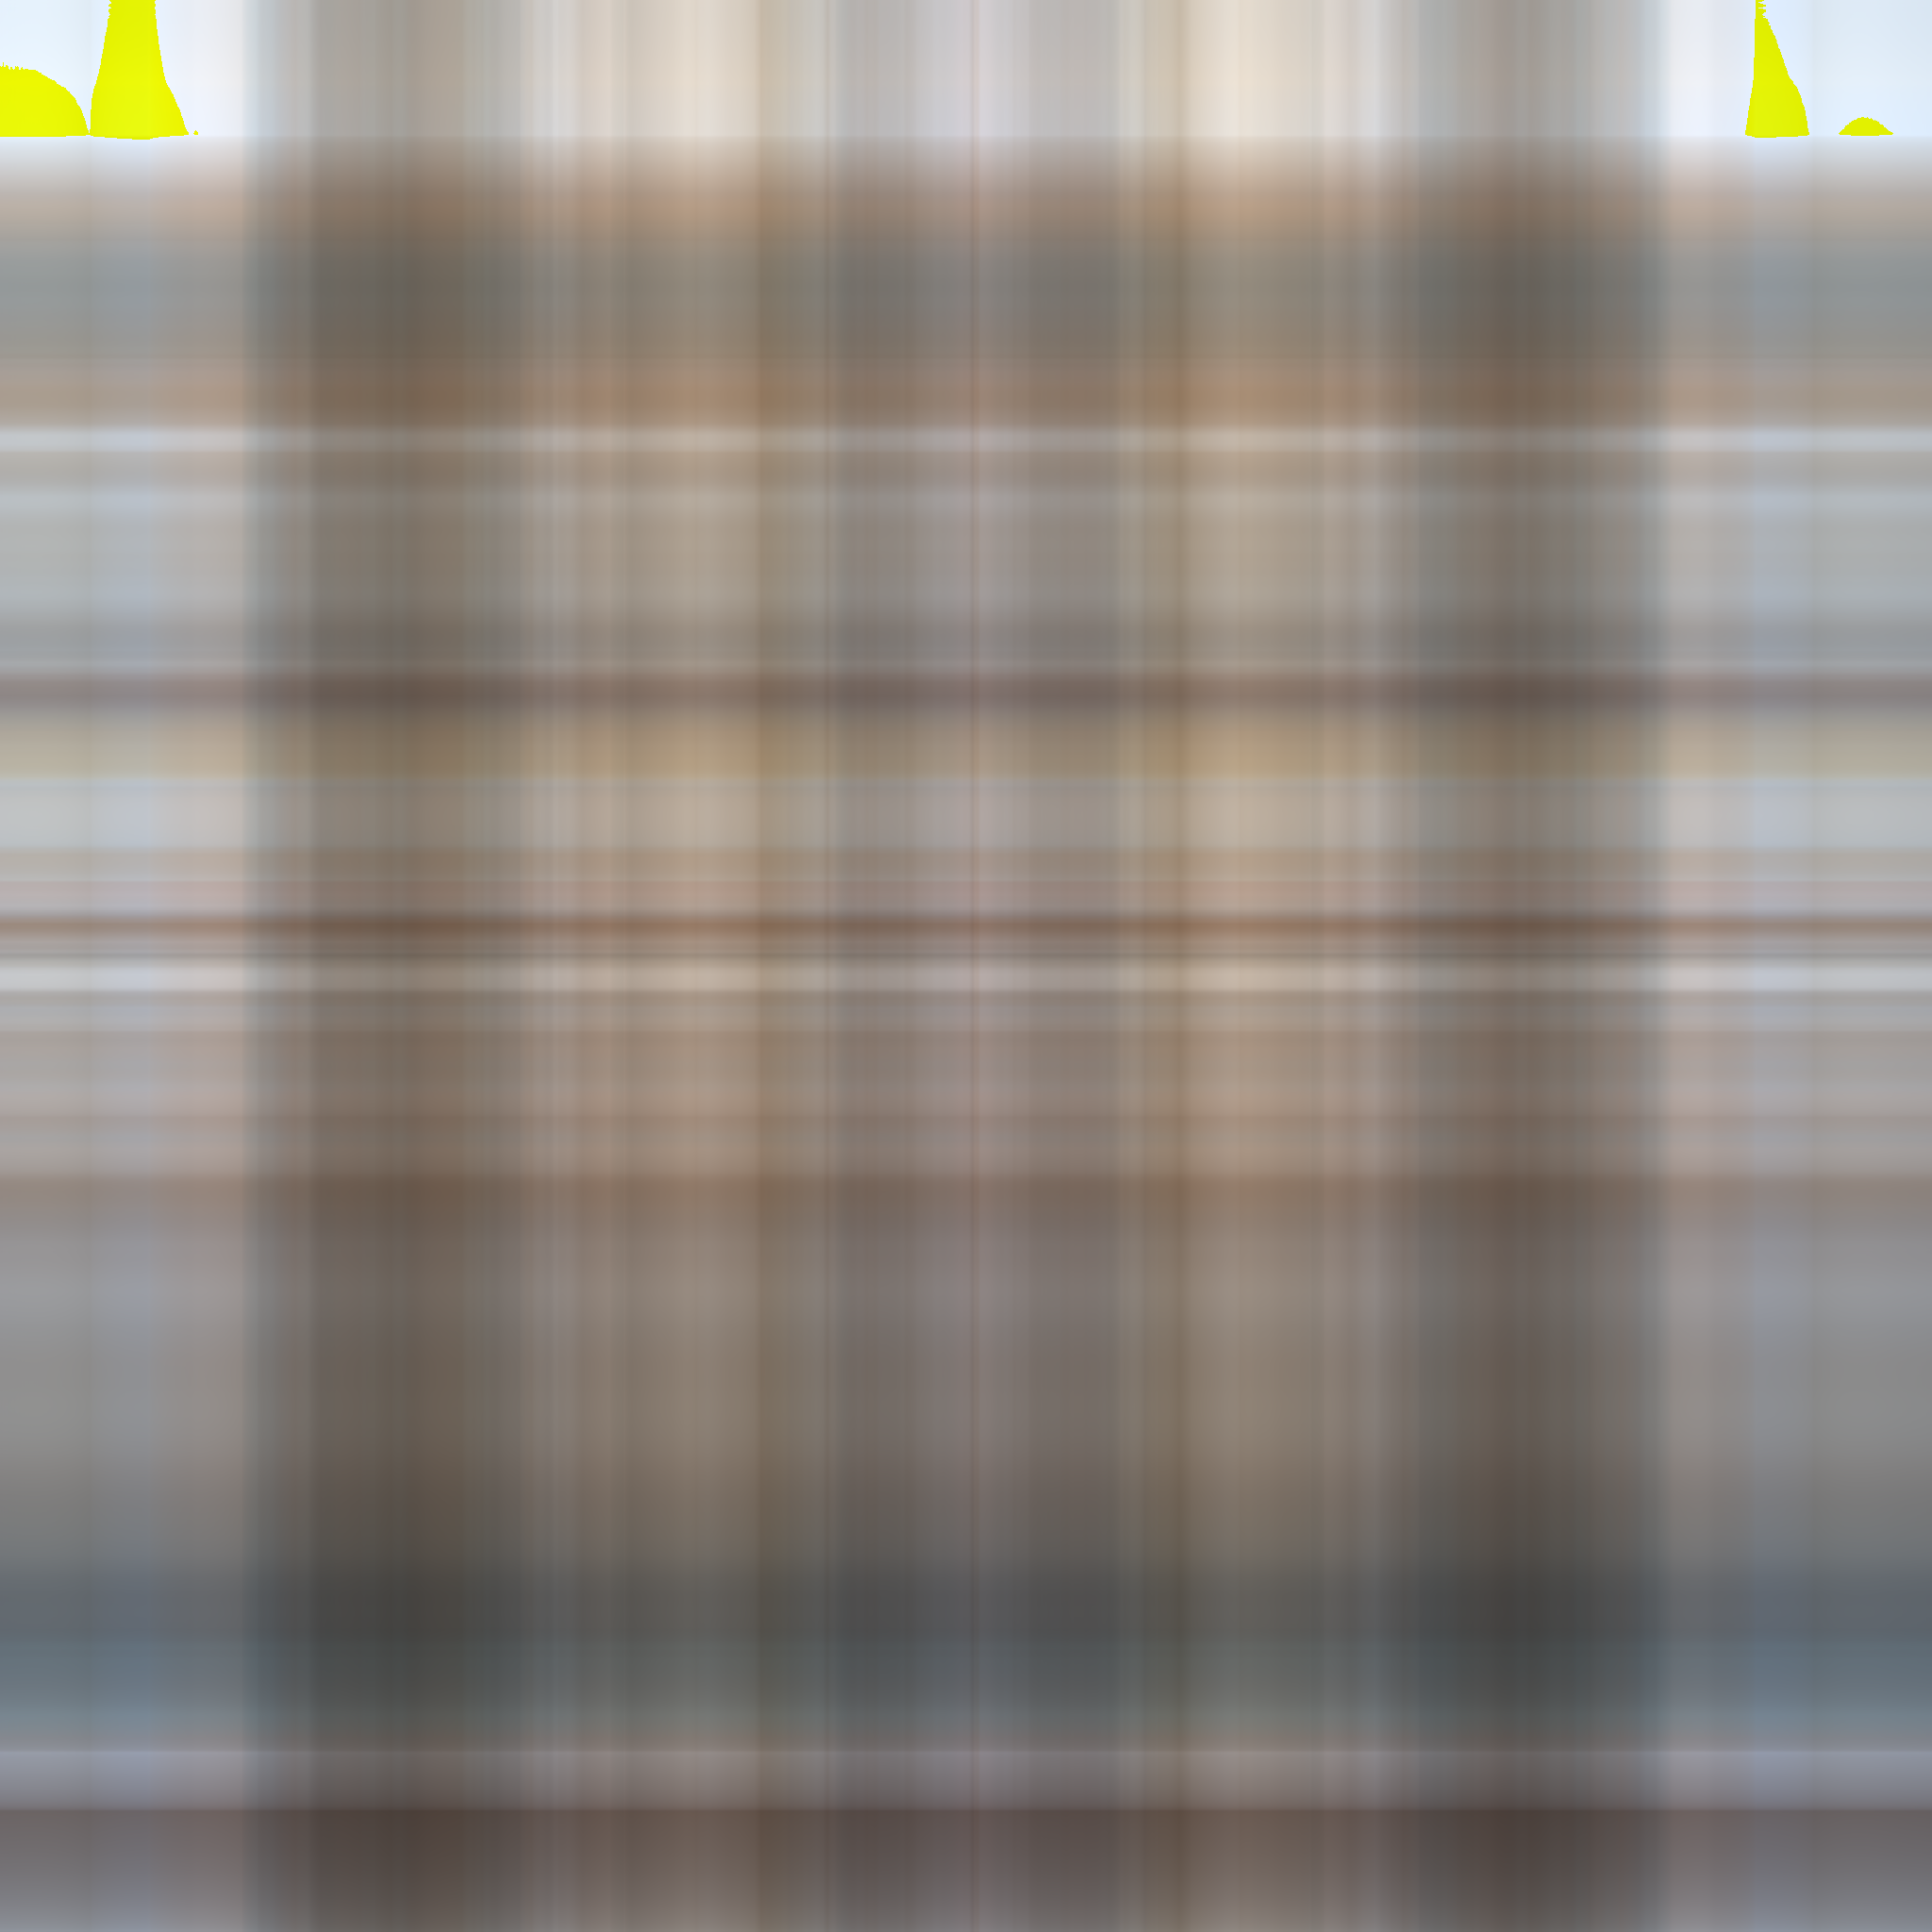
\includegraphics[width=\linewidth]{../image-compression-color/cat-1.png}
  \caption{$rank=1$}
  \label{fig:cat-bw-rank-1}
\end{figure}

\begin{figure}
  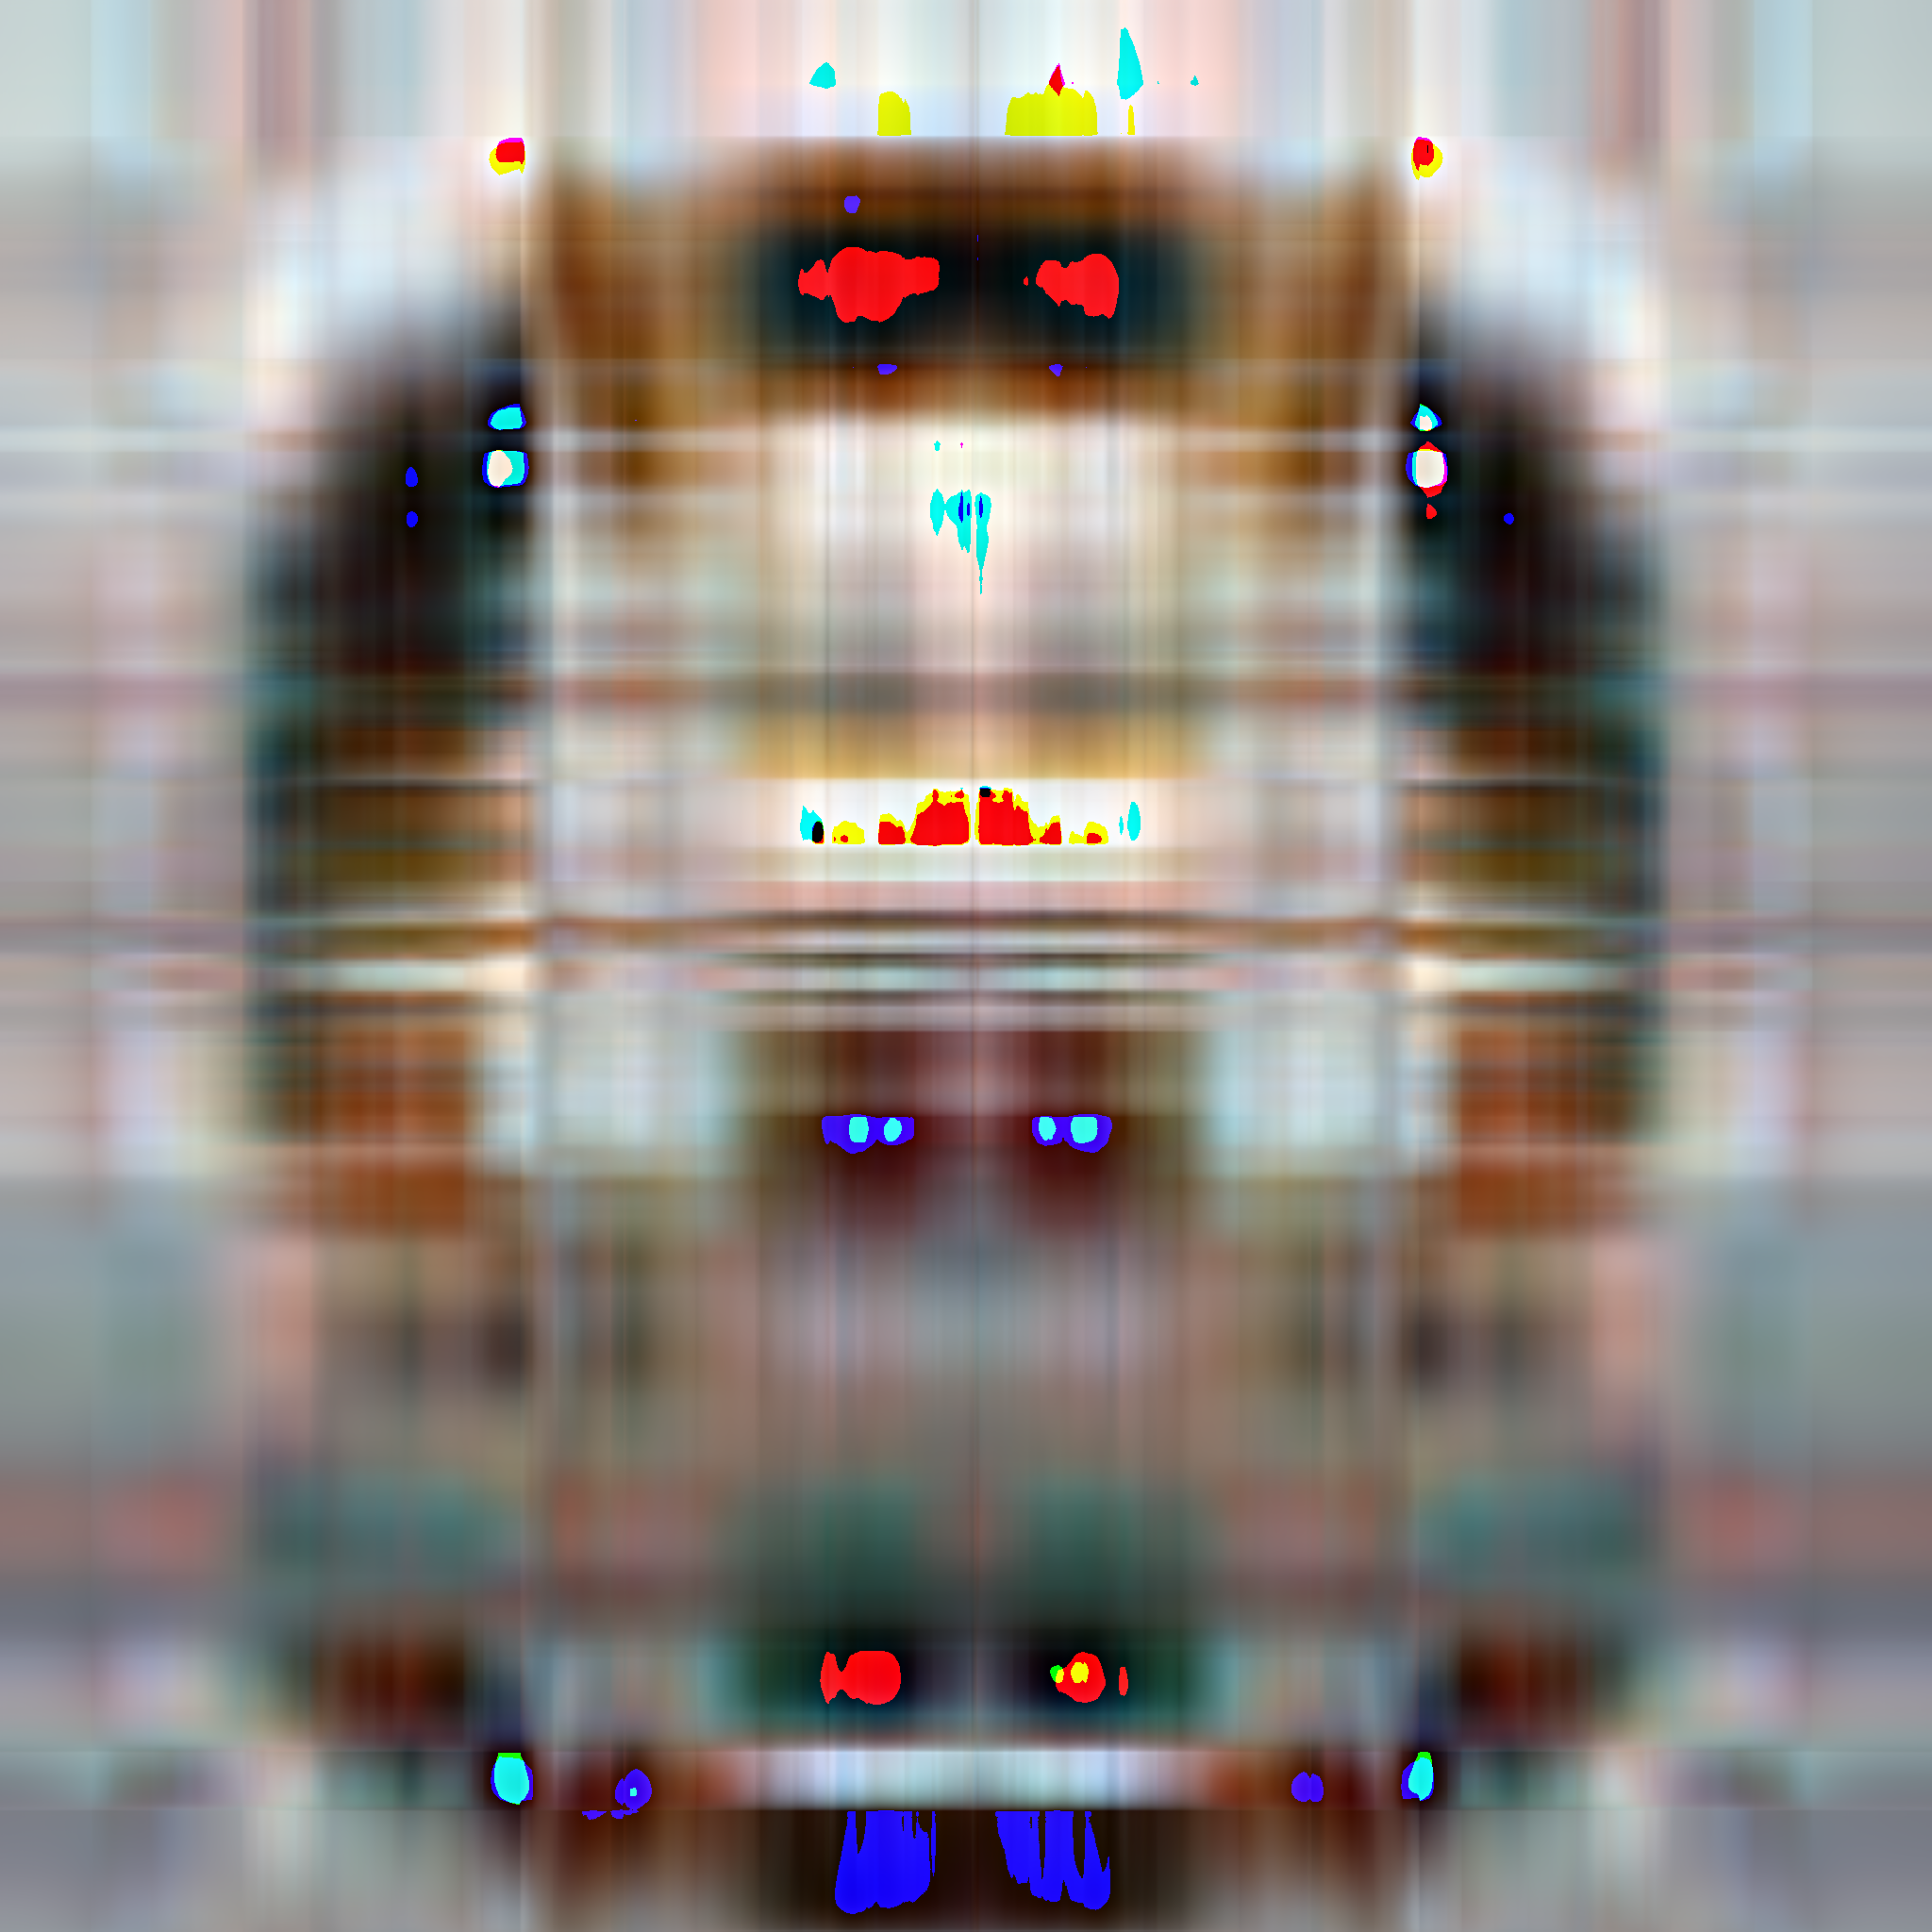
\includegraphics[width=\linewidth]{../image-compression-color/cat-4.png}
  \caption{$rank=4$}
  \label{fig:cat-bw-rank-4}
\end{figure}

\begin{figure}
  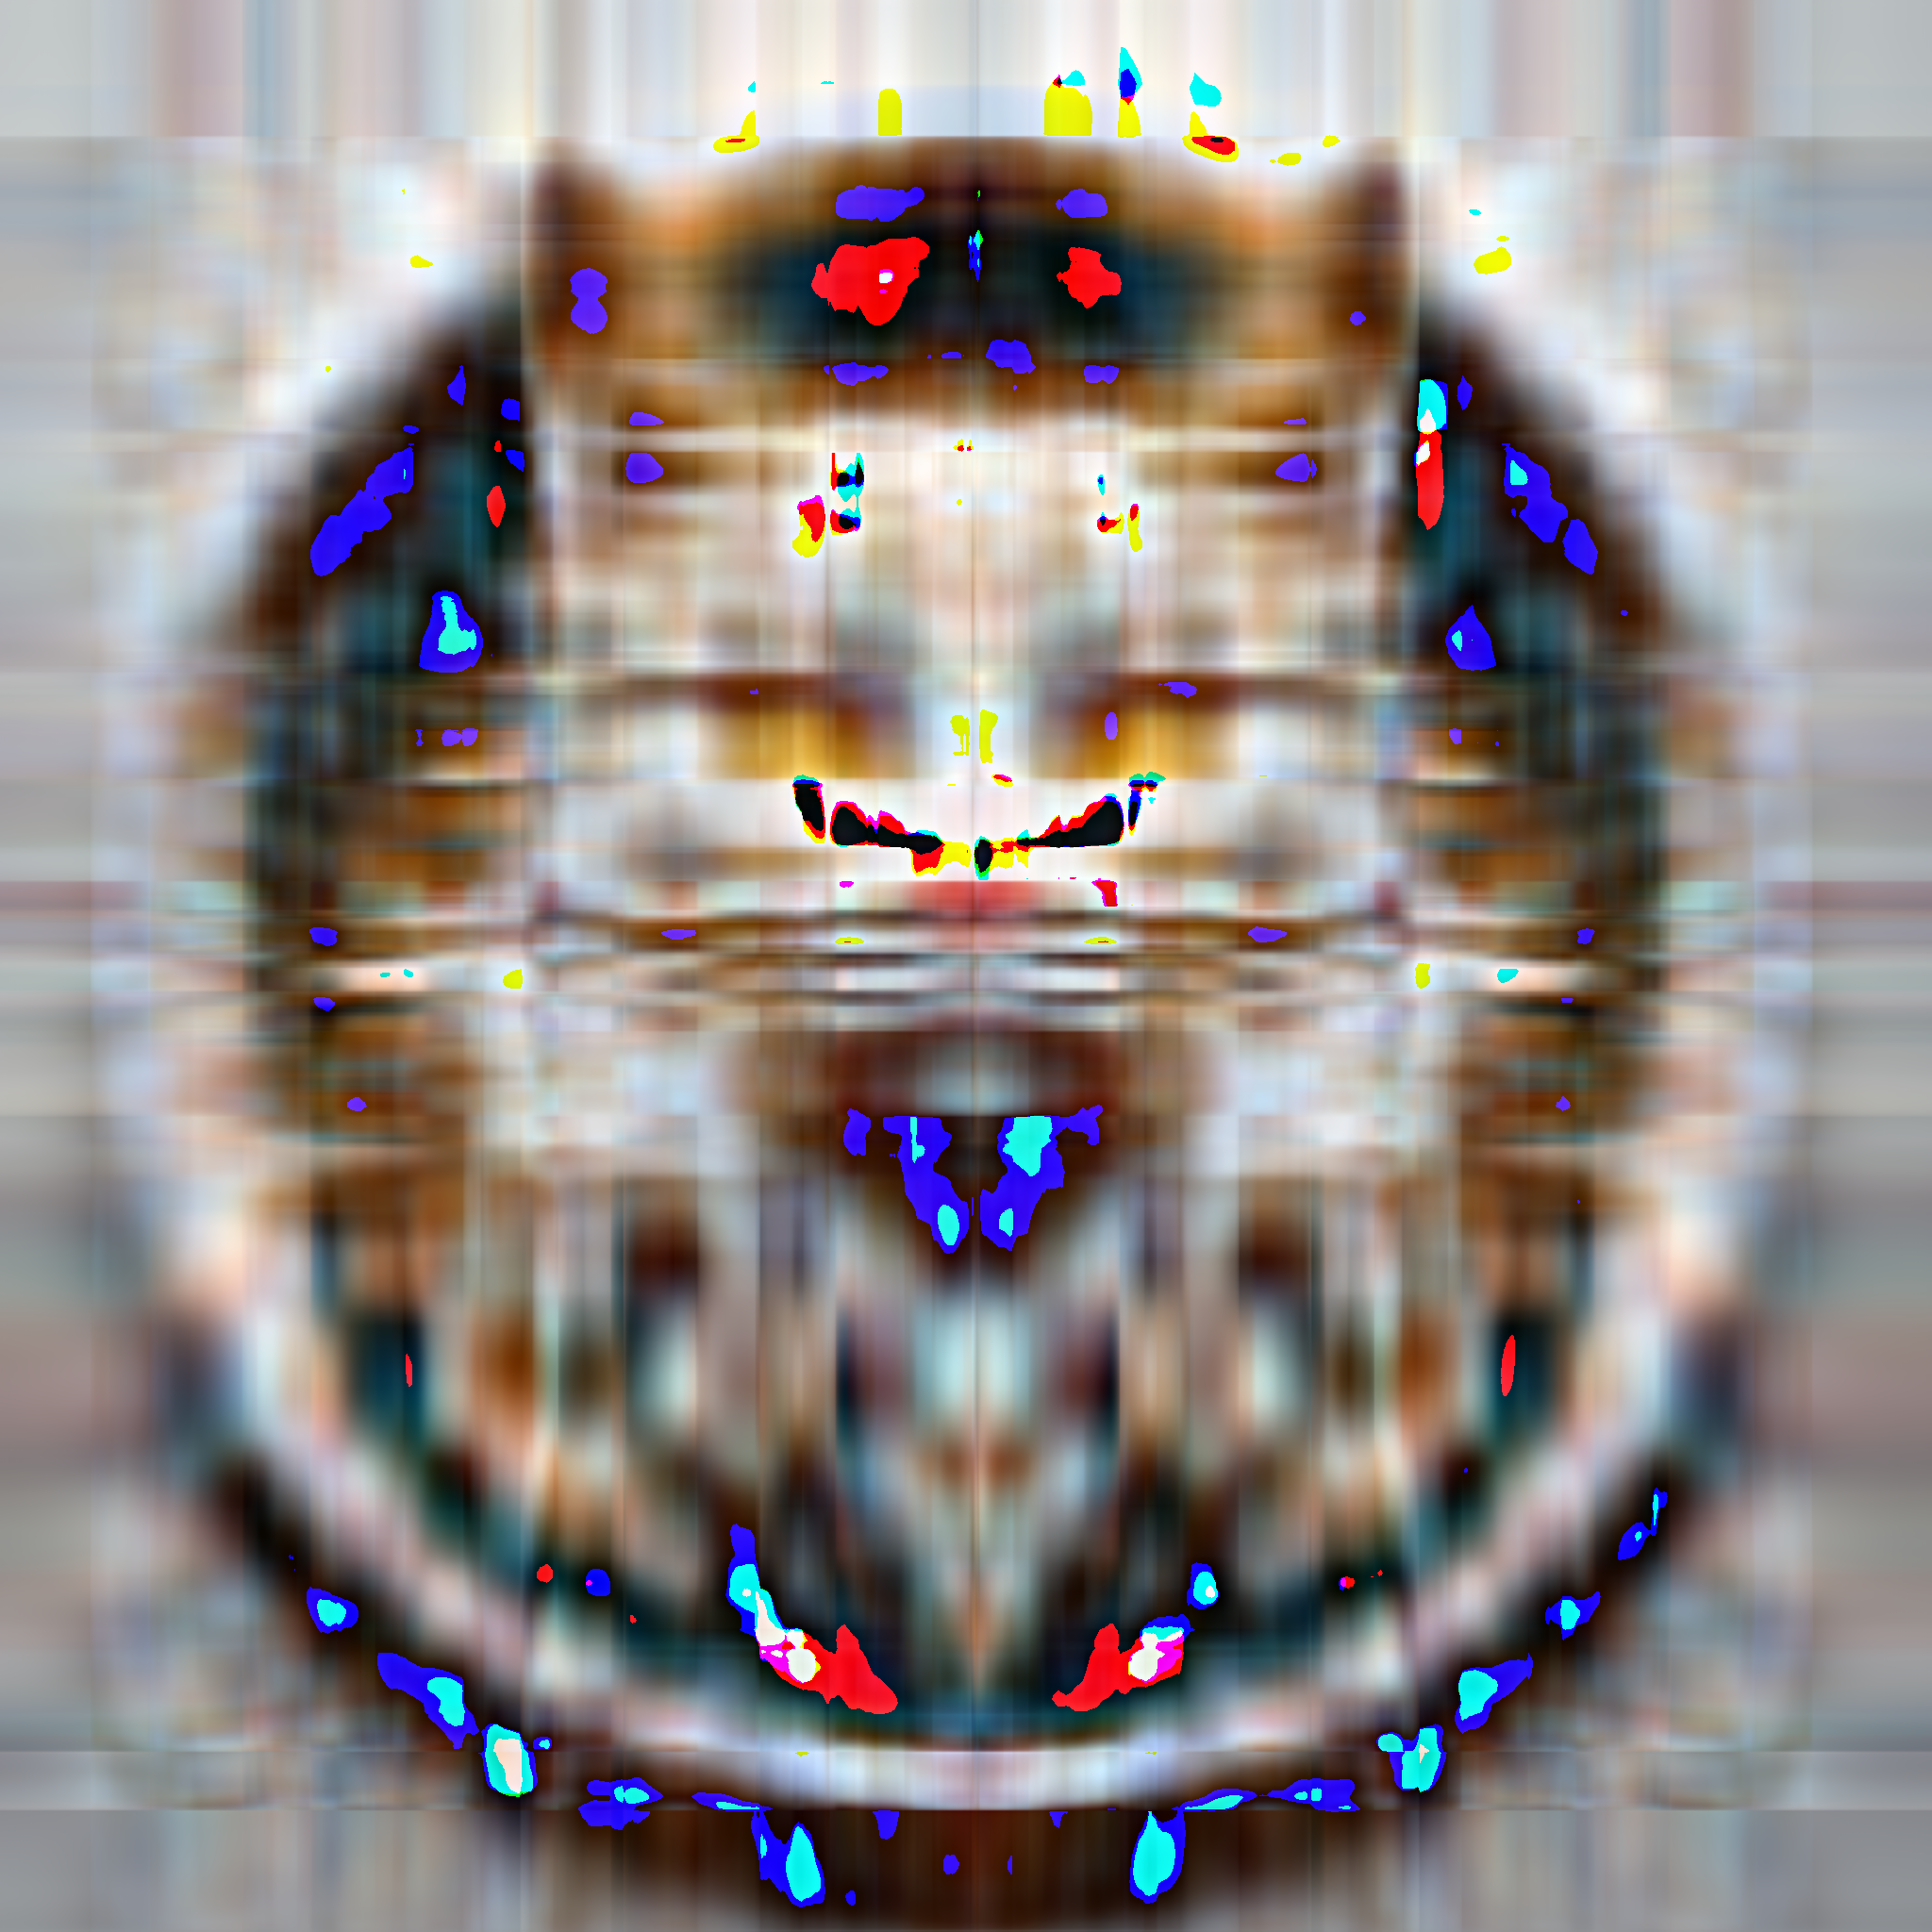
\includegraphics[width=\linewidth]{../image-compression-color/cat-8.png}
  \caption{$rank=8$}
  \label{fig:cat-bw-rank-8}
\end{figure}

\begin{figure}
  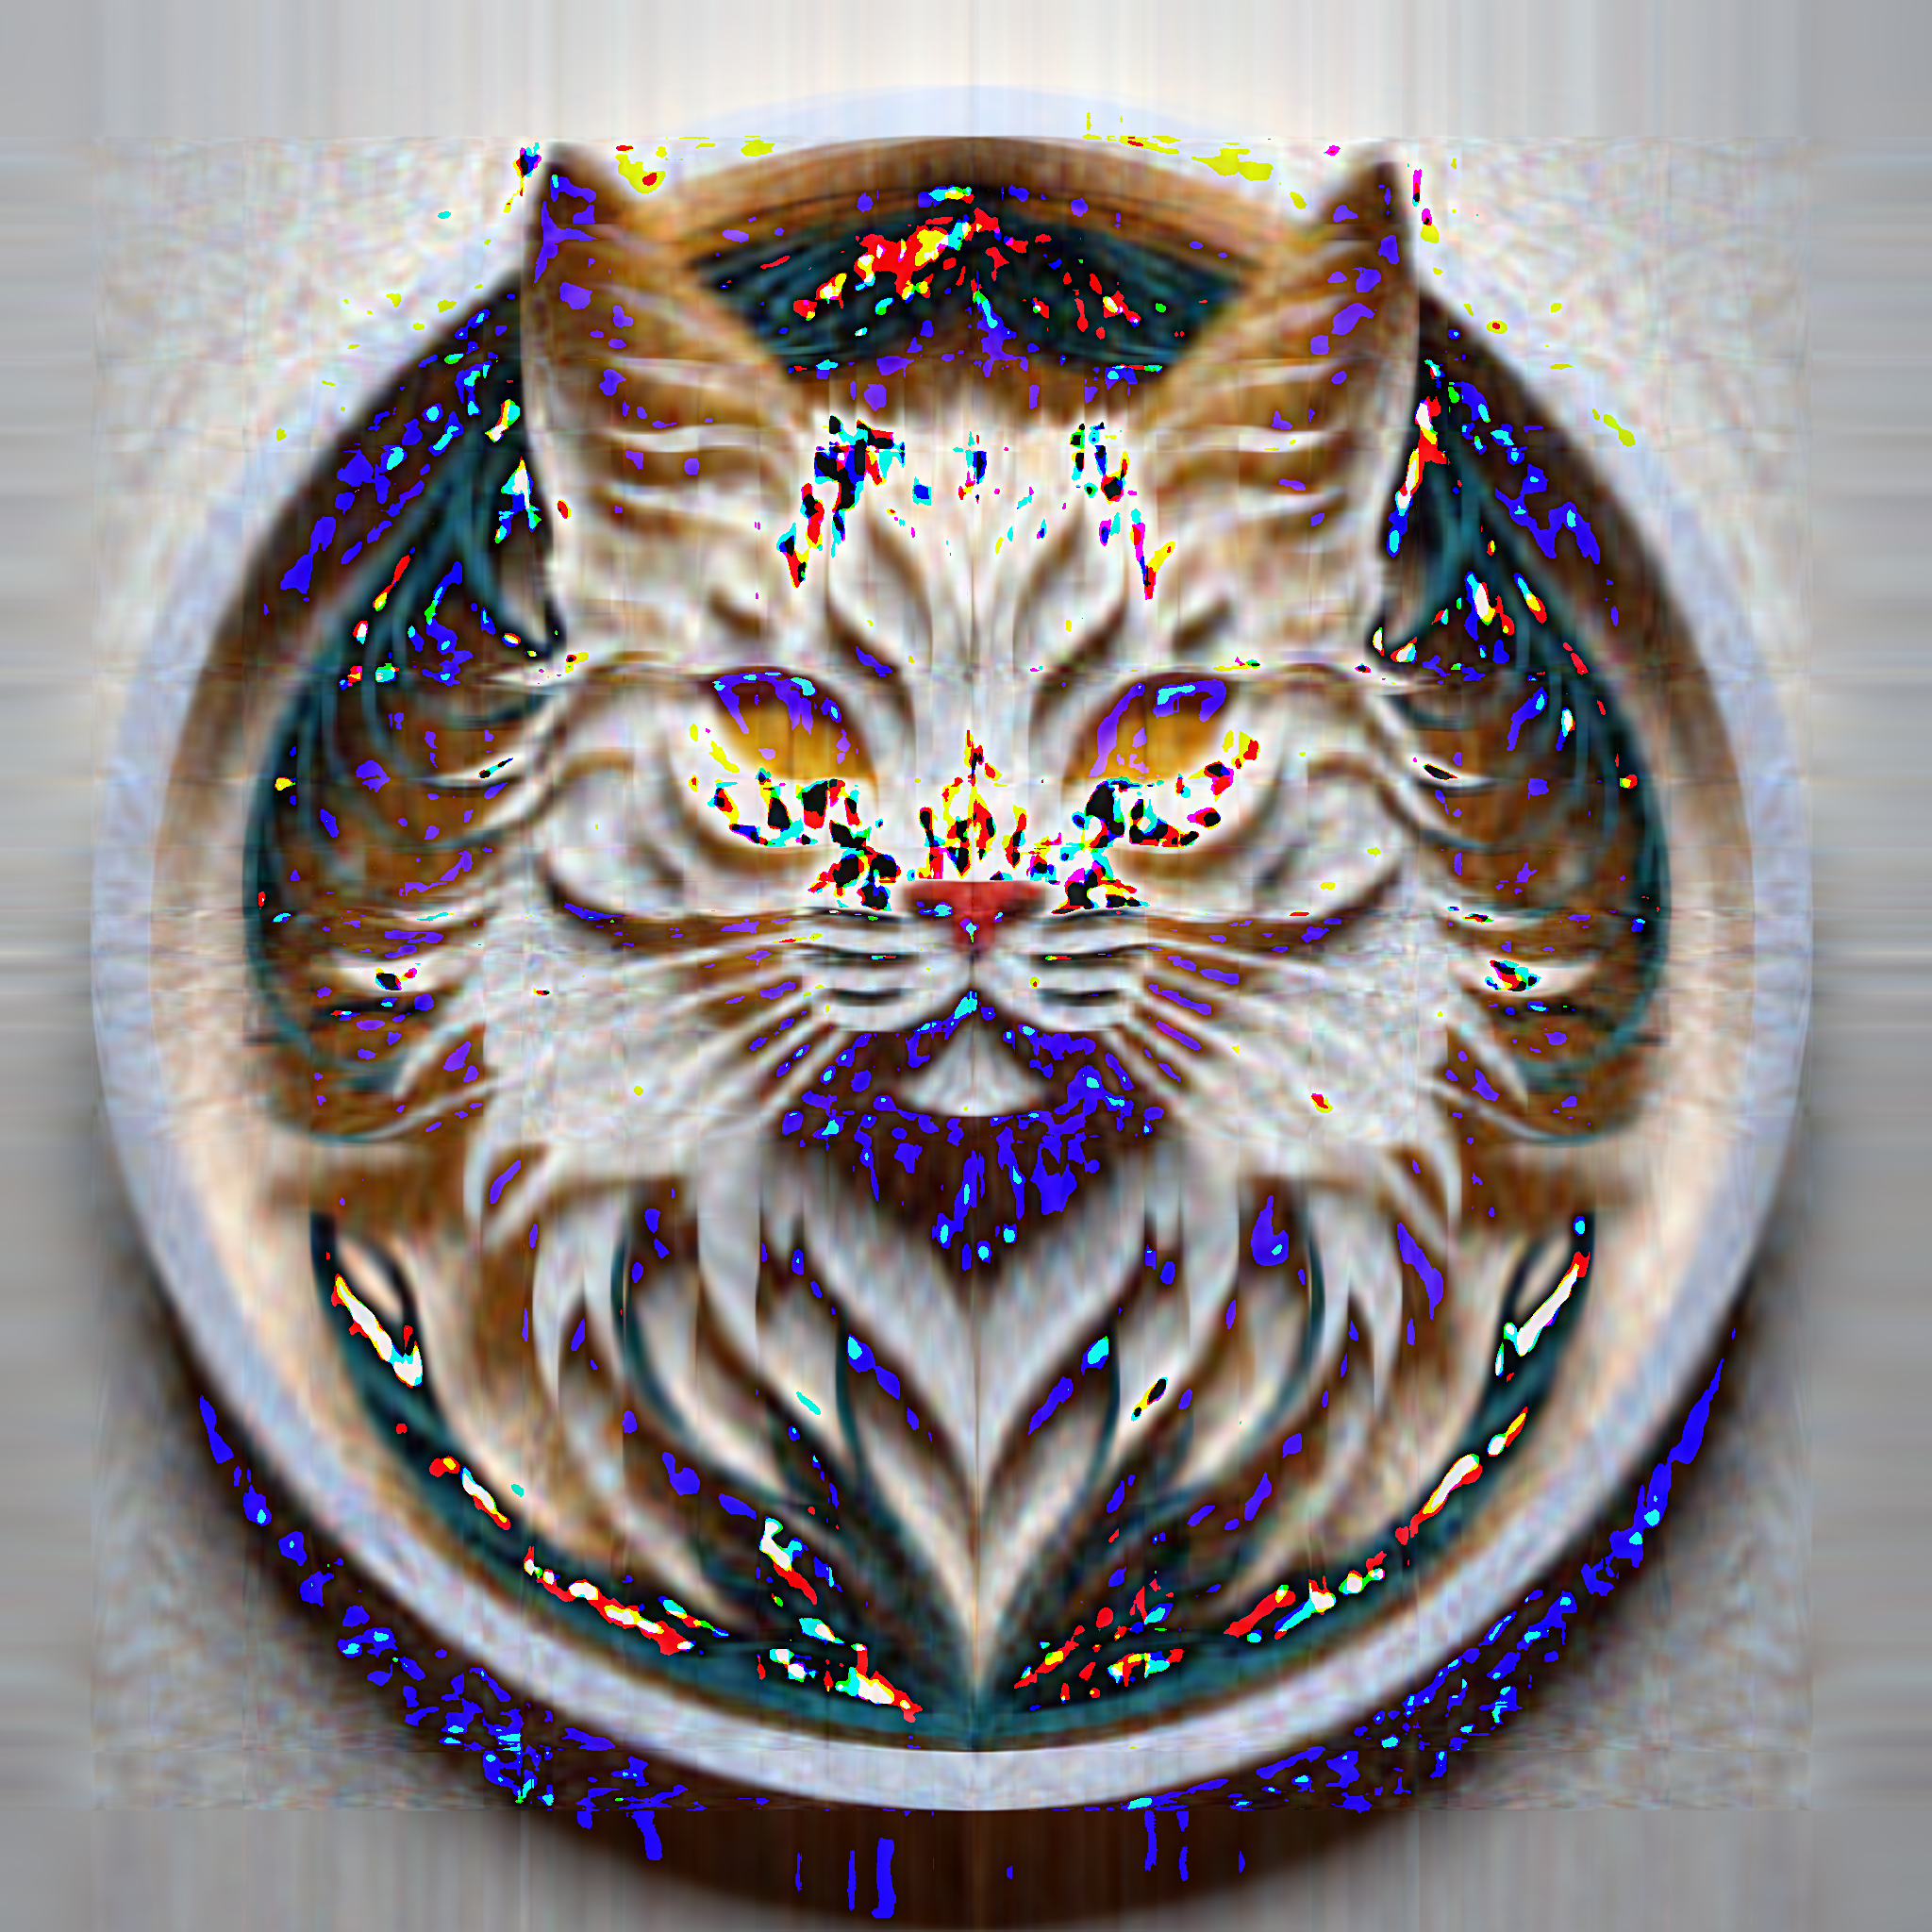
\includegraphics[width=\linewidth]{../image-compression-color/cat-32.png}
  \caption{$rank=32$}
  \label{fig:cat-bw-rank-32}
\end{figure}


\begin{figure}
  \includegraphics[width=\linewidth]{../image-compression-color/cat-256.png}
  \caption{$rank=256$}
  \label{fig:cat-bw-rank-256}
\end{figure}


\begin{figure}
  \includegraphics[width=\linewidth]{../image-compression-color/cat-1024.png}
  \caption{$rank=1024$}
  \label{fig:cat-bw-rank-1024}
\end{figure}

\begin{figure}
  \includegraphics[width=\linewidth]{../image-compression-color/cat-2048.png}
  \caption{$rank=2048$}
  \label{fig:cat-bw-rank-2048}
\end{figure}

\insertfig{../output/image-comp-col-mse.pgf}{\lr{MSE vs Rank}}{bw_comp_col_mse}
\insertfig{../output/image-comp-col-mse-log.pgf}{\lr{MSE vs log Rank}}{bw_comp_col_mse_log}
\insertfig{../output/image-comp-col-psnr.pgf}{\lr{PSNR vs Rank}}{bw_comp_col_psnr}
\insertfig{../output/image-comp-col-psnr-log.pgf}{\lr{PSNR vs log Rank}}{bw_comp_col_psnr_log}
